% !TeX root=_main_.tex
% chapter4

\chapter{روش پیشنهادی}\label{ch:4}
\thispagestyle{empty}


\epigraph{
	«اولین قانون هر فناوری مورد استفاده در یک کسب‌وکار این است که اِعمال خودکارسازی به یک عملیات کارآمد، کارآمدی را افزایش می‌دهد. دومین قانون این است که اِعمال خودکارسازی به یک عملیات ناکارآمد، ناکارآمدی را افزایش می‌دهد.»
}
{$ \maltese $ {\large بیل گیتس}}

\noindent
هدف، در روش پیشنهادی همان‌طور که پیش‌ از این هم گفته شد، ایجاد یک مدل برای یادگیری خودکار گرامر قالب فایل و سپس استفاده از آن در تولید داده‌های آزمون جدید است. معماری مدل یادگیرنده ساختار فایل، نحوه آموزش، مجموعه داده لازم برای آموزش مدل، نحوه تولید داده‌های آزمون و در نهایت چگونگی انجام آزمون فازی، مباحثی هستند که در این فصل به آنها خواهیم پرداخت. در ابتدا به بیان کلیات روش پیشنهادی پرداخته و سپس هریک از مراحل را با جزئیات تشریح می‌کنیم.


\section{کلیات}
شکل \ref{ch4_zakeri_proposed_method_flowchart_crop.pdf} یک روندنمای ساده از کلیات مراحل انجام روش پیشنهادی ما را نشان می‌دهد. در ساختار برخی قالب‌های فایل پیچیده مانند \gls{PDF}، بسیاری از قسمت‌ها به صورت متنی هستند. اما ممکن است قسمت‌های دودویی هم وجود داشته باشد. در روش پیشنهادی خود ما ابتدا کلیه قسمت‌های متنی فایل‌های موجود در دانه‌های اولیه را استخراج، سپس این قسمت‌ها را به یکدیگر الحاق می‌کنیم. حاصل این کار ایجاد یک \gls{Corpus} بزرگ است که در بطن خود مشخصه‌های قالب یک فایل را دارد. در ادامه این مجموعه را مطابق با ضوابط فنون یادگیری ماشینی به سه مجموعه آموزش، ارزیابی و آزمون تقسیم‌بندی با نسبت‌های مشخص می‌کنیم. سپس یک مدل مولد را ایجاد و آن را روی داده‌های مجموعه آموزش، با تعریف یک روش یادگیری، آموزش می‌دهیم. در نهایت از این مدل برای ایجاد داده‌های آزمون جدید و اعمال آزمون فازی استفاده خواهیم کرد. اما چون مدل صرفاً قادر به تولید داده‌های متنی است در هنگام ایجاد یک داده آزمون، با فنونی که در ادامه خواهیم گفت، قسمت‌های دودویی را نیز به داده آزمون تزریق می‌نماییم. 


%% برای رعایت قاعده ارجاع به جلو بایستی از پرچم ht در محیط‌های شناور لاتک استفاده کرد.
% h means here: Place the figure in the text where the figure environment is written.
% t means top: Place it at the top of a page.
% b means bottom: Place it at the bottom of a page.
% p means page: Place it on a page containing only floats.
\begin{figure}%[ht]%[tbh!]%%[t!]
	\centering
	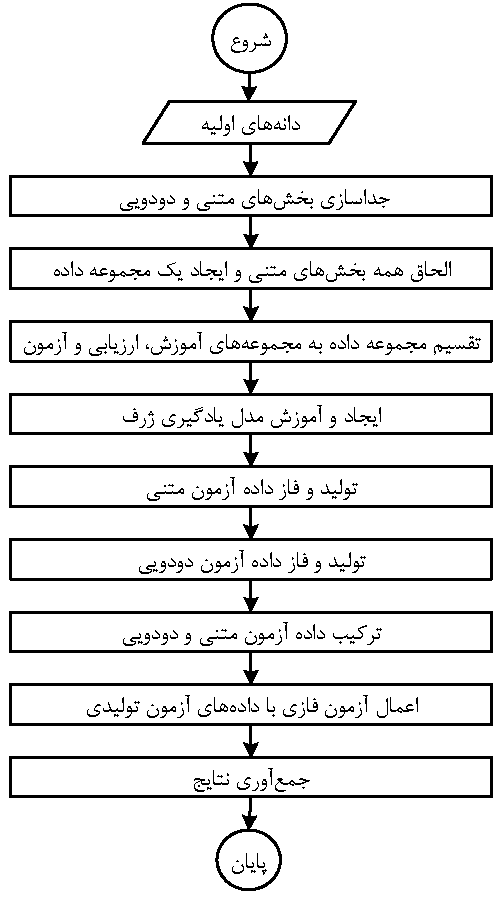
\includegraphics[width=0.7\textwidth, clip=true,  trim= 0 0 0 0]{chapter4/ch4_zakeri_proposed_method_flowchart_crop.pdf}
	%\includegraphics[width=\textwidth]{figs/chapter1/ch1_fuzz_testing_flowchart2.png}
	\caption[روندنمای روش پیشنهادی در حالت کلی]
	{
		روندنمای روش پیشنهادی در حالت کلی.
	}
	\label{ch4_zakeri_proposed_method_flowchart_crop.pdf}
	%\ref{ch4_zakeri_proposed_method_flowchart_crop.pdf}
\end{figure}


\subsection{تمایز داده‌های متنی و دودویی}
گفتیم مدل مولد را روی بخش متنی قالب فایل ایجاد می‌کنیم. اما مفهوم دقیق متنی و دودویی و معیار جداسازی آنها چیست و دلیل تأکید ما بر این موضوع از کجا نشئت می‌گیرد؟ منظور از داده‌های متنی در اینجا مجموعه کدهای \gls{ASCII} است. هنگامی که درسطح بیت یک فایل را بررسی می‌کنیم تمایزی میان واژه‌های متنی و دودویی نیست؛ زیرا همه چیز با مفهوم صفر و یک بیان می‌شود که دودویی است. اما اگر فایل را به‌صورت یک توالی از بایت‌ها در نظر بگیریم، با توجه به اینکه هر بایت 255 حالت ممکن خواهد داشت، می‌توانیم آن فایل را یک زبان متشکل از تکرار حداکثر 255 نشانه بدانیم. کدهای  \gls{ASCII} حتی این تعداد را به 128 نشانه که کاراکترها و نشانه‌های متداول زبان انگلیسی هستند، محدود می‌کنند. مشکل بخش‌های دودویی آن است که اغلب در سطح بیت تفسیر می‌شوند و یادگیری وابستگی‌های آنها با شبکه‌های عصبی، که داده‌های محدودی را در زمان آموزش می‌بینند، امکان‌پذیر نیست. از طرفی هنگامی که نسبت کوچکی از داده‌ها به‌صورت دودویی در میان قسمت‌های متنی ظاهر می‌شوند می‌توان آنها را با روش‌های جابه‌جایی تصادفی فاز کرد.

ما در روش پیشنهادی خود داده‌های دودویی را از قالب فایل حذف کرده اما به‌جای آن یک توکن خاص موسوم به \gls{BinaryToken} را جایگزین می‌کنیم. بدین ترتیب در فرایند آموزش مدل توزیع آماری نحوه ظاهر شدن قسمت‌های دودویی نیز فراگیری می‌شود. حال در فرایند تولید داده‌های آزمون جدید مدل مکان‌های احتمالی ظاهر شدن قسمت دودویی را با پیش‌بینی وقوع توکن مربوطه، تعیین می‌کند. سپس توکن را با یک قسمت دودویی که به‌صورت تصادفی (یا هر روش دیگر) فاز شده است جایگزین می‌کنیم. یعنی وارون عملی که پیش از فرایند آموزش انجام دادیم را پس از فرایند تولید، انجام می‌دهیم. با کلیت گفته شده در اینجا یک روش ترکیبی تولید خودکار داده آزمون خواهیم داشت.


\subsection{تمایز داده و فراداده}\label{sec:data_and_metadata}
در فصل \ref{chapter1}، تمایز داده و فراداده به عنوان یک مسئله در تولید داده آزمون مطرح گردید. مدل مطرح در روش پیشنهادی این امکان را فراهم می‌کند تا بتوانیم به‌صورت احتمالی داده و فراداده را از یکدیگر تشخیص دهیم. از آنجایی که فراداده‌ها در ساختار یک فایل از پیش‌ تعریف شده و تقریباً ثابت هستند، تکرار آنها به مراتب بیشتر از تکرار داده‌ها است که محتویات یک فایل را تشکیل می‌دهند. مدل بدین ترتیب در توزیع آماری یادگیری شده احتمال بیشتری را به فراداده‌ها نسبت می‌دهد. با تعیین یک آستانه مشخص برای هریک از انواع داده و فراداده در هنگام تولید داده آزمون قادر به تصمیم‌گیری در مورد نوع آنها هستیم. ما نتیجه این تصمیم را در نحوه فاز داده آزمون جدید به‌کار می‌بریم، بدین صورت که دو الگوریتم فاز با اهداف فاز فراداده برای مرحله تجزیه و فاز داده برای مرحله پرداخت فایل ارائه خواهیم داد.     


\subsection{مثال انگیزشی}
تمرکز اصلی ما در روش پیشنهادی، بر روی پیمانه تولید داده آزمون در یک فازر قالب فایل است. شکل \ref{ch4_motivating_example}، مراحل تولید داده آزمون از طریق روش پیشنهادی را روی قالب فایل \lr{PDF}، نشان می‌دهد. سه مرحله اصلی در این شکل وجود دارد که به ترتیب با شماره‌های یک تا سه، شماره‌گذاری شده‌اند. مطابق این مراحل، ابتدا پیکره‌ای از فایل‌های از پیش موجود و معتبر جمع آوری گردیده و به عنوان مجموعه داده انتخاب می‌شوند. در مرحله اول، یعنی پیش‌پردازش، هریک از فایل‌های ورودی پیمایش شده، بخش‌های متنی آن جدا و به یکدیگر الحاق می‌شوند. همچنین بخش‌های دودویی داخل فایل، نیز به‌صورت مجزا، پس از جدا شدن، نگهداری می‌شوند. در فایل \lr{PDF}، بخش‌هایی دودویی بین کلیدواژه‌های 
\lr{stream} و \lr{endstream}
می‌آیند که در پیش‌پردازش آنها را با توکن دودویی 
\lr{stream}
جایگزین می‌کنیم. خروجی این مرحله دو مجموعه است. یک مجموعه داده متنی و یک مجموعه داده دودویی. در مجموعه داده متنی، مکان قسمت‌های دودویی با توکن دودویی مشخص شده است.

در مرحله دوم، یک مدل زبانی عصبی برروی مجموعه داده حاصل از جداسازی بخش‌های متنی پیکره آموزش داده می‌شود. مانند هر وظیفه یادگیری ماشینی در این مرحله ابتدا مجموعه داده ورودی به سه مجموعه آموزش، آزمون و ارزیابی تقسیم می‌گردد. خروجی این مرحله یک مدل مولد است که قادر به تولید داده‌های جدید با پیروی از توزیع حاکم بر داده‌های مجموعه آموزش بوده و کاراکتر به کاراکتر داده‌های جدید را تولید می‌کند.

مرحله سوم با روش‌هایی اقدام به تولید داده‌های آزمون جدید، در این‌جا فایل‌های 
\lr{PDF}،
می‌کند. در این مرحله بخش‌های متنی فایل جدید از طریق مدل مولد، یعنی با روش مبتنی بر تولید، ایجاد می‌گردد. عمل بدشکل کردن داده‌های متنی نیز همزمان با تولید آنها صورت می‌گیرد. بدین صورت که برخی از کاراکترها بعد از تولید، بر اساس شرایطی که در ادامه فصل توضیح داده می‌شوند، با کاراکترهای دیگری جایگزین می‌شوند. در همین مرحله، بخش‌هایی دودویی نیز در صورت پیش‌بینی توسط مدل مولد، با یک روش مبتنی بر جابه‌جایی، تولید و در مکان مناسب خود قرار می‌گیرند. منظور از پیش‌بینی در اینجا، تولید توکن دودویی 
\lr{stream}
در توسط مدل مولد است. در تولید بخش دودویی یک داده‌ آزمون از بخش‌های دودویی پیکره اولیه که در مرحله یک جداسازی شده است به‌عنوان دانه اولیه استفاده می‌کنیم. در واقع آنها را با یکی از عملگر‌های جابه‌جایی که در فصل 
\ref{chapter2}
 به آن اشاره شد به‌سادگی جابه‌جا کرده و یک داده آزمون دودویی جدید و فاز شده می‌سازیم. 

مرحله سوم در مجموع تعدادی داده آزمون را با روشی ترکیبی، تولید می‌کند. این داده‌های آزمون سپس می‌توانند به عنوان داده‌های آزمون در فرایند آزمون فازی استفاده شوند. همچنین می‌توان از آن به عنوان دانه اولیه برای فازرهای قالب فایل مبتنی بر جابه‌جایی نیز استفاده کرد. برای ارزیابی روش پیشنهادی خود که در فصل بعد به آن خواهیم پرداخت، در انتهای این فصل یک فازر قالب فایل ساده را مطرح می‌کنیم. این فازر قادر است تا پس از تولید داده‌های آزمون به روش شرح داده شده آنها را به عنوان ورودی به 
\gls{SUT}
تزریق کرده و خطاهای احتمالی را در صورت وجود گزارش کند. مرحله پیش‌پردازش بسیار ساده بوده و نیاز به توضیح خاصی ندارد. این مرحله ممکن است برای قالب‌های فایل مختلف، کاملاً متفاوت باشد. مثلاً برای قالب‌های فایل متنی مثل
\lr{HTML}و \lr{XML}
پیش‌پردازش تنها الحاق کردن کلیه فایل‌های موجود در پیکره است. مراحل دوم و سوم، یعنی ایجاد و آموزش مدل مولد و تولید و فاز داده آزمون، به ترتیب در بخش 
\ref{sec:model}
 و بخش 
 \ref{sec:neural_fuzzing_algorithms}
 توضیح داده شده‌اند. همچنین معماری فازر قالب فایل پیشنهادی در بخش 
 \ref{sec:implementation}
 %\sethlcolor{cyan}\hl{بیان شده است.}
بیان گردیده است.


 

\begin{figure}
	\centering
	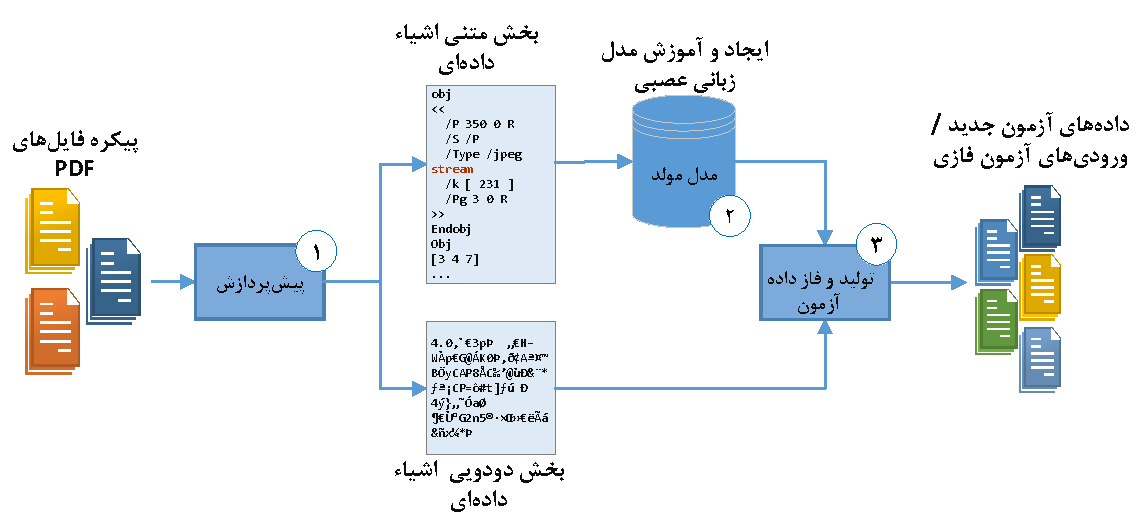
\includegraphics[width=1.0\textwidth, clip=true,  trim= 0 0 0 0]{chapter4/ch4_motivating_example_crop.pdf}
	\caption[مراحل یادگیری ساختار فایل، تولید و فاز داده آزمون برای فایل \lr{PDF}]
	{
		مراحل یادگیری ساختار فایل، تولید و فاز داده آزمون برای فایل \lr{PDF}. 
	}
	\label{ch4_motivating_example}
	%\ref{ch4_motivating_example}
\end{figure}


\section{مدل}\label{sec:model}
یک فایل را می‌توان نمونه تولید شده توسط زبانی که قالب آن فایل را بیان می‌کند دانست. با این فرض می‌توان یک مدل زبانی برای هر قالب فایلی ایجاد کرد. مدل زبانی عصبی عملکرد بهتری نسبت به مد‌های زبانی سنتی دارد. با توجه به ذات مبتنی بر توالی بایت‌های یک فایل، وابستگی بایت فعلی به یک توالی از بایت‌‌های قبلی و نیز تجزیه ترتیبی (چپ به راست و بالا به پایین) آن توسط تجزیه‌گر \gls{SUT} در بسیاری از موارد، در روش پیشنهادی خود، از \gls{RNN} برای ایجاد مدل زبانی و یادگیری ساختار فایل استفاده می‌کنیم. در فصل \ref{chapter2} دیدیم که \gls{RNN} برای یادگیری وظایف مبتنی بر توالی ابداع شده است. به‌طور دقیق‌تر در هنگام آموزش از یک مدل \gls{RNN} چند به یک، با معماری شکل \ref{ch2_karpathy_rnn_crop.pdf} (پ) استفاده خواهیم کرد و در هنگام تولید داده‌ جدید با فراخوانی همین مدل به‌صورت متوالی، مدلی از نوع شکل \ref{ch2_karpathy_rnn_crop.pdf} (ت) خواهیم داشت.

هدف \gls{RNN} در اینجا ایجاد یک مدل زبانی عصبی روی ساختار فایل با دیدن یک پیکره از نمونه‌های آموزشی است. مطابق آنچه گفتیم، مدل زبانی مدلی مولد است، یعنی پس از آموزش، می‌توان از آن برای تولید داده‌های آزمون جدید استفاده کرد، که در ادامه نحوه این کار را توضیح خواهیم داد. در این پایان‌نامه دو مدل با معماری مختلف بر مبنای \gls{RNN} می‌سازیم. در هسته عصب‌های \gls{RNN} هر دو مدل از سلول \gls{LSTM} استفاده می‌کنیم که قابلیت یادگیری توالی‌های با طول زیاد را دارد. مدل اول \gls{LSTM} \gls{Unidirectional} نام دارد که معماری آن مشابه شکل \ref{ch2_rnn.pdf} است. مدل دوم \gls{LSTM} \gls{Bidirectional} است.

\gls{LSTM}
دوسویه توالی ورودی را به دو صورت \gls{Forward} و  \gls{Backward} می‌بیند. در واقع \gls{LSTM} \gls{Bidirectional} از دو \gls{LSTM} یک‌سویه تشکیل شده است. یکی از آنها توالی را از چپ به راست پردازش می‌کند و دیگری از راست به چپ. در نتیجه هر گذرجلو \gls{LSTM} دو خروجی خواهد داشت. یک \gls{MergeFunction} برای ادغام خروجی هریک از \gls{LSTM}های روبه‌جلو و روبه‌عقب به‌کار می‌رود. \gls{MergeFunction} می‌تواند هر تابعی که قادر به ترکیب دو بردار با طول‌های یکسان است، درنظر گرفته شود؛ از جمله: جمع، ضرب، الحاق و غیره. ما از \gls{MergeFunction} جمع برای مدل پیشنهادی خود استفاده می‌کنیم که درایه‌های نظیر به نظیر هر یک از بردارهای خروجی را با یکدیگر جمع می‌زند.

علاوه‌بر نوع مدل \gls{LSTM}، برای \gls{LSTM} یک‌سویه مدل‌هایی با تعداد عصب‌های متفاوت و نیز تعداد لایه‌های پنهان متفاوت را ساخته‌ایم. هدف از این کار مشاهده تأثیر مدل‌های با پیچیدگی مختلف در یادگیری ساختار فایل و تولید داده‌های آزمون و آزمایش این فرضیه است که آیا مدل‌های پیچیده‌تر، مدل‌های ساده‌تر را شکست می‌دهند؟ یعنی موفق به افزایش پوشش کد و یا شناسایی خطاهای بیشتری می‌شوند یا خیر. جـدول \ref{tabel:deep_model} مدل‌های طراحی شده برای استفاده در آزمایش‌های روش پیشنهادی و مشخصه‌های هریک را نشان می‌دهد. یکی از مهم‌ترین مشخصه‌ها تعداد پارامترهای هر مدل است. گراف محاسباتی هریک از مدل‌های جدول \ref{tabel:deep_model} در شکل‌های \ref{ch4_keras_model_archs_crop.pdf}الف تا \ref{ch4_keras_model_archs_crop.pdf}ت آمده است. اندازه ماتریس‌های ورودی و خروجی در گراف مرتبط با تعداد لایه‌های پنهان و نیز تعداد عصب‌ها در هر لایه است که در ادامه بیشتر توضیح داده خواهد شد. همچنین در ادامه پایان‌نامه، هریک از مدل‌های معرفی شده، با شماره ذکر شده برای آنها در جدول 
\ref{tabel:deep_model}
شناخته می‌شوند.

\begin{table}%[ht]
	\caption{مدل‌های یادگیری ژرف طراحی شده، پارامترها و ابرپارامترهای آنها.}
	\label{tabel:deep_model}
	\centering
	\onehalfspacing
	\begin{tabularx}{\textwidth}{r l r r r}
		
		\toprule[1.5pt] شماره (نام) مدل 
		& نوع (معماری) مدل 
		& تعداد لایه  پنهان
		 & تعداد عصب در هر لایه
		  & تعداد پارامترها
		\\
 		\midrule[1.5pt] 1 &  \makecell[l]{\lr{Unidirectional LSTM} \\ \lr{(Many to One)}} & 1 & 128 & 127584
 		\\
 		%\hline 
 		2 & \makecell[l]{\lr{Unidirectional LSTM} \\ \lr{(Many to One)}} & 2 & 128 & 238656
 		\\
 		%\hline 
 		3 & \makecell[l]{\lr{Unidirectional LSTM} \\ \lr{(Many to One)}} & 2 & 256 & 870464
 		\\
 		%\hline 
 		4 & \makecell[l]{\lr{Bidirectional LSTM} \\ \lr{(Many to One)}} & 2 & 128 & 469056
 		\\
 		\bottomrule[1.5pt]
 
	\end{tabularx} 
\end{table}


\begin{figure}%[ht]%[tbh!]%%[t!]
	\centering
	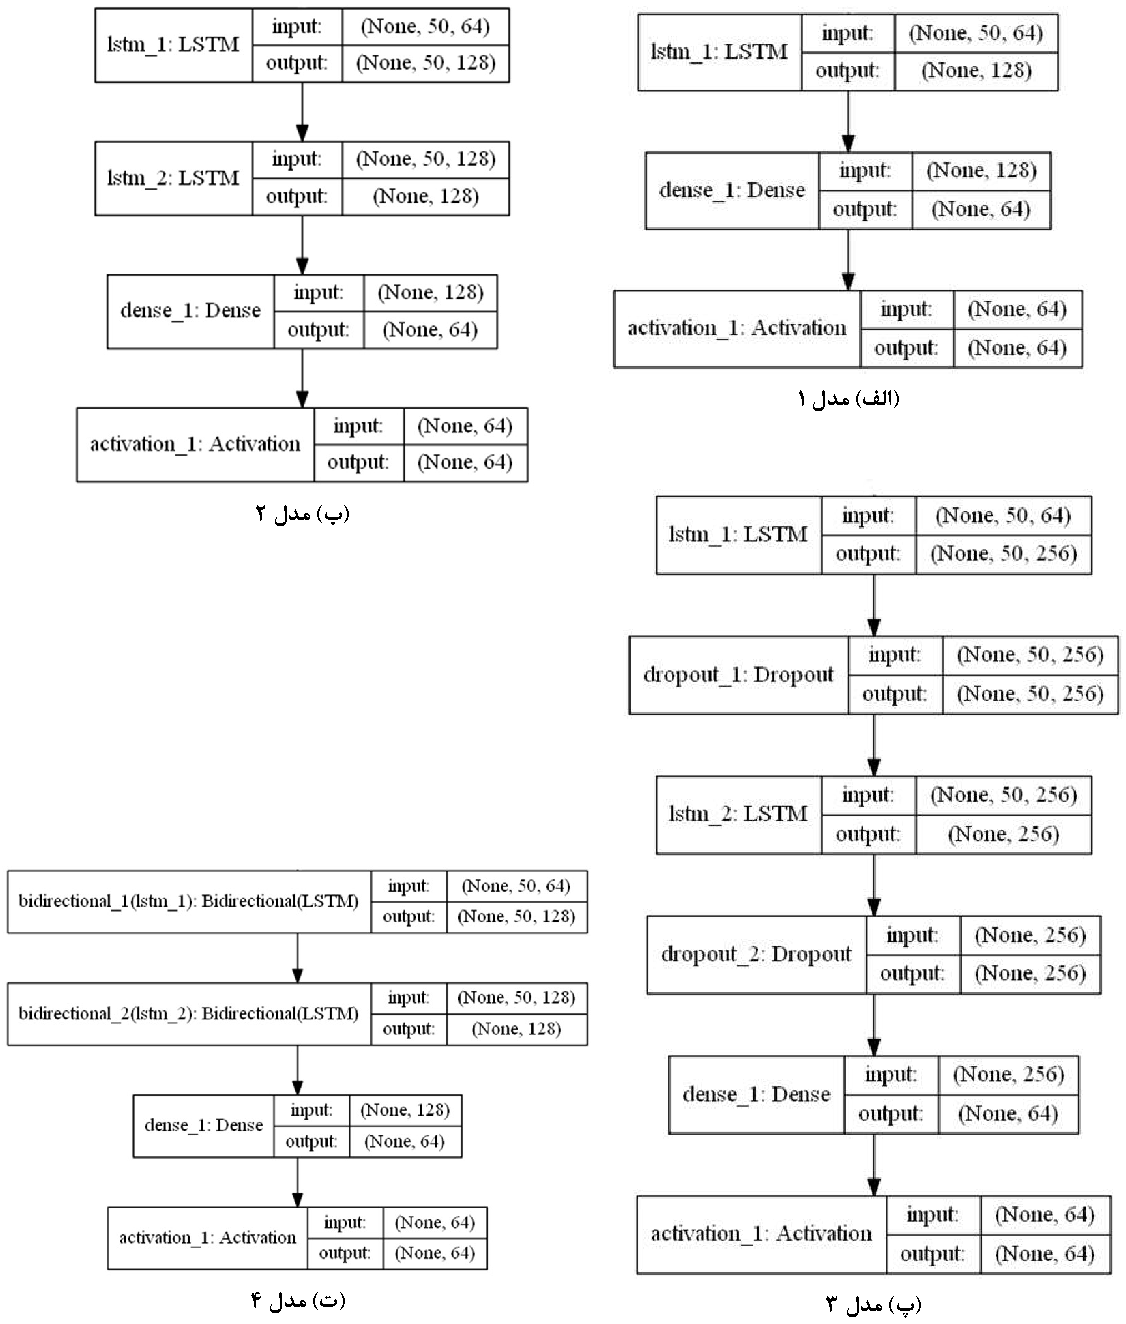
\includegraphics[width=\textwidth, clip=true,  trim= 0 0 0 0]{chapter4/ch4_keras_model_archs_crop.pdf}
	\caption[گراف محاسباتی مدل‌های عصبی ژرف جدول \ref{tabel:deep_model}]
	{
		گراف محاسباتی مدل‌های عصبی ژرف جدول \ref{tabel:deep_model}. اعداد داخل مستطیل‌ها اندازه ماتریس‌های ورودی و خروجی هر لایه را نشان می‌دهند. گراف‌ها با استفاده از توابع کتابخانه \lr{Keras} \cite{chollet2015keras} تولید شده‌اند.  
	}
	\label{ch4_keras_model_archs_crop.pdf}
	%\ref{ch4_keras_model_archs_crop.pdf}
\end{figure}



\subsection{آموزش مدل}

فرایند آموزش همه مدل‌های جدول \ref{tabel:deep_model} یکسان است. در واقع برای آموزش هر مدل تنها نیاز داریم که ورودی و خروجی شبکه عصبی ژرف را مشخص نماییم. پس از استخراج مجموعه داده اولیه که حاوی یک پیکره متوالی از کاراکترهای در بردارنده فایل است، آن را به مجموعه‌های آموزش، آزمون و ارزیابی تقسیم می‌کنیم. چون خروجی مدل مولد در هربار اجرا یک توالی خواهد بود، طول توالی‌های مجموعه داده معیار مناسبی برای تقسیم‌بندی آن به مجموعه‌های سه‌گانه یاد شده است به ‌نحوی که هر مجموعه توزیع یکسانی از فراوانی طول‌های مختلف باشد. از مجموعه‌های آموزش و ارزیابی در هنگام آموزش مدل و از مجموعه آزمون در هنگام تولید داده‌های جدید از روی مدل، استفاده خواهیم کرد. تفکیک مجموعه داده به سه مجموعه آموزش، ارزیابی و آزمون در وظایف یادگیری ماشینی یک امر بدیهی است، اما استفاده از آن برای آزمون فازی و تولید داده‌های آزمون جدید تا قبل از این، انجام نشده و چنان‌چه در ادامه خواهیم دید، ایده جدیدی است. در واقع ما از داده‌های مجموعه آزمون برای تولید داده‌های آزمون جدید استفاده خواهیم کرد.

هر مجموعه بدین ترتیب حاوی تعدادی فایل است و هر فایل یک توالی از کاراکتر‌های \lr{ASCII} است. شروع و پایان هریک از این توالی‌ها پیش از فرایند آموزش، با توکن‌های شروع و پایان که نشانه‌های مجزایی (بیرون از مجموعه داده) هستند برچسب‌گذاری‌ می‌شود. البته بسیاری از قالب‌های فایل چنین توکن‌هایی را به‌عنوان بخشی از ساختار خود دارند. برای مثال فایل‌های \lr{HTML} با برچسب $ <html> $ شروع و با برچسب $ </html> $ خاتمه می‌یابند. فایل‌های \lr{XML} و \lr{PHP} نیز چنین هستند. در این حالت نیازی به افزودن توکن‌های شروع و پایان جدید نیست و می‌توان از همین توکن‌ها استفاده کرد. دلیل افزودن توکن‌های شروع و پایان در این مرحله، به نحوه ساخت مدل‌های زبانی عصبی باز‌ می‌گردد. در واقع این مدل‌ها با دیدن توکن آغازین پیش‌بینی را شروع و با تولید توکن پایانی، پیش‌بینی را خاتمه می‌دهند.

%دلیل این امر همان‌طور که در بخش \ref{sec:language_model} دیدیم، نحوه ساخت مدل‌های زبانی با استفاده از شبکه‌های عصبی است.  

به‌منظور آموزش هر مدل چند به یک و ایجاد یک مدل زبانی عصبی، ابتدا با الحاق محتوای فایل‌های مجموعه آموزش، یک توالی بزرگ از کاراکترها به‌شکل  
$ S = <s^{(1)}, s^{(2)}, s^{(3)}, ..., s^{(n)}> $
 ایجاد می‌کنیم. سپس این توالی را به تعدادی توالی ورودی کوچکتر با طول ثابت $ d $ می‌شکنیم طوری که $i$امین توالی ورودی برابر است با:
 \begin{equation}\label{rel:input_sec}
 	x_i=S[i*j:(i*j)+d]
 \end{equation}
  
  در رابطه 
  \ref{rel:input_sec}،
  $s[l,u]$
   برشی از توالی $s$ بین شاخص‌های $l$ و $u$ بوده و $j$ میزان پرش به جلو در انتخاب توالی ورودی بعدی از توالی اصلی را نشان می‌دهد. ابرپارامتر $d$
   در اینجا، در واقع همان بردار زمینه در مدل زبانی است.
   انتخاب $d$ به پارامترهایی مانند فاصله وابستگی‌های بین بایت‌های مختلف در یک فایل و طول فایل‌های مجموعه‌ داده، بستگی دارد. وقتی از 
   \gls{LSTM}
   به عنوان بلوک‌های سازنده 
   \gls{RNN}
   در ساخت 
   \gls{NLM}
   استفاده شود، می‌توان وابستگی‌های طولانی‌تر را به خوبی یاد‌ گرفت. 
   در عمل و برای وظایف مدل زبانی، این مقدار را بین 40 تا 100 نشانه در نظر می‌گیرند.
   
   گفتیم شبکه عصبی در حالت بانظارت آموزش می‌بیند؛ یعنی، برای هر ورودی یک برچسب خروجی نیاز است. در اینجا کاراکتر بعدی، که هدف پیش‌بینی آن است، را به عنوان برچسب خروجی برای هر توالی ورودی نسبت می‌دهیم. بنابراین برچسب خروجی برای $i$امین توالی ورودی برابر خواهد بود با:
   \begin{equation}
   	 Y_{x_{i}} = S[(i*j) + d+1]
   \end{equation}
     
     
     پس از تولید همه نمونه‌های آموزشی و برچسب‌های متناظر آنها، مدل به صورت انتهابه‌انتها  %\LTRfootnote{\lr{End-to-End}}
     آموزش داده می‌شود؛ مشابه روش یادگیری و فاز
     \cite{Godefroid:2017:LML:3155562.3155573}.
     . یعنی، داده‌های خام مجموعه آموزش، بدون استخراج هیچ‌گونه ویژگی خاصی به شبکه داده می‌شوند و در زمان استفاده نیز، شبکه داده‌های نهایی را بدون نیاز به هیچگونه پسا‌پردازشی تولید می‌کند. در این حالت مدل قادر پیش‌بینی مقدار احتمال شرطی 
     $p(x^{(i+d+1)}| <x^{(i)}, ..., x^{(i+d)}>)$
     خواهد بود. روند تولید نمونه‌های آموزشی در الگوریتم \ref{alg:produce_training_samples} نشان داده شده است. همچنین شکل \ref{ch4_html_toy_example_crop.pdf}، یک فایل \lr{HTML} و سه‌توالی آموزشی اول تولید شده برای آن توسط الگوریتم \ref{alg:produce_training_samples} را به همراه موقعیت قرارگیری آنها در شبکه نشان می‌دهد. توالی ورودی کلی در این مثال، همه کاراکترهای فایل \lr{HTML} و پارامترهای $d$  و $j$ به‌ترتیب برابر 3 و 1 قرار داده شده‌اند. مقادیر در نظر گرفته شده کاملاً فرضی هستند.

شبکه عصبی با مقادیر عددی کار می‌کند. بنابراین بایستی یک نمایش عددی برای هر کاراکتر در مجموعه آموزش در نظر گرفت. یک روش مرسوم در مدل‌های مبتنی بر کاراکتر استفاده از بردارسازی \lr{One-hot} یا $1$ از $k$ است. در این روش یک بردار به  طول اندازه مجموعه واژگان برای هر کاراکتر درنظر می‌گیرند که تنها یکی از شاخص‌های آن برابر $1$ است. بدین ترتیب برای نمایش $V$ کاراکتر، $V$ بردار متفاوت خواهیم داشت. در اینجا نیز از همین روش استفاده می‌کنیم. 

خروجی شبکه نیز که به‌شکل یک کاراکتر تعریف شده است در واقع یک بردار \lr{One-hot} است. در فرایند آموزش تنها یکی از شاخص‌های این بردار یک است. اما در مرحله آزمون بردار تولیدی حاوی مقادیر حقیقی مختلفی در بازه
 $(-\infty, +\infty)$
  برای هر شاخص است. با اعمال تابع بیشینه هموار (رجوع شود به رابطه \ref{softmaxformula})، در خروجی این لایه، می‌توان خروجی را به یک توزیع احتمالی معتبر تبدیل کرد.


\begin{algorithm}%[ht]
	\onehalfspacing
	\caption{\lr{ProduceTrainingSamples}} \label{alg:produce_training_samples}
	\begin{latin}
		\DontPrintSemicolon
		\setcounter{AlgoLine}{0}
		\LinesNumbered
		
		\SetKwFunction{List}{List} 
		\SetKwFunction{Len}{Len} 

		
		\SetKwInput{KwData}{Input}
		\SetKwInput{KwResult}{Output}
		
		\KwData{Total sequence $S$, Input sequences lenght $d$, Jump step $j$}
		\KwResult{Input sequences $x$, Output labels $Y$}
		
		\BlankLine
		
		$x$ $\gets$	\List{} \tcc*{Make an empty list}\; 
		
		$Y$ $\gets$ \List{} \tcc*{Make an empty list}\;
		
		\For{$i \gets 1$ \KwTo \Len{$S$} $ - d $ }{
			
			$x[i] \gets S[i*j:(i*j)+d]$
		
			$Y[i] \gets S[(i*j) + d+1]$
		
	}
	\textbf{Return}	$x$, $Y$

	\end{latin}
\end{algorithm}


\begin{figure}%[ht]%[tbh!]%%[t!]
	\centering
	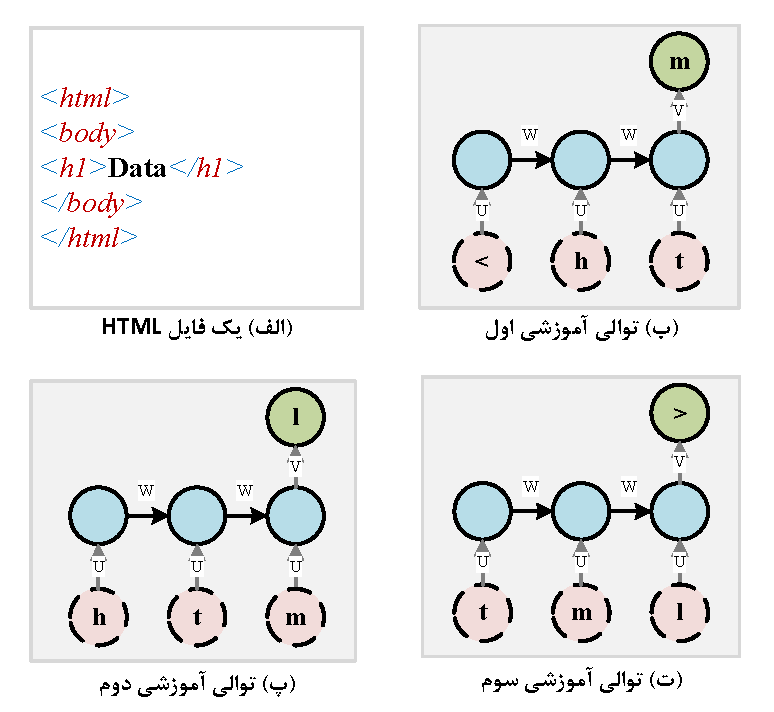
\includegraphics[width=0.95\textwidth, clip=true,  trim= 0 0 0 0]{chapter4/ch4_html_toy_example_crop.pdf}
	\caption[مثالی از نحوه آموزش مدل‌های چند به یک]
	{
		مثالی از نحوه آموزش مدل‌های چند به یک روی یک فایل \lr{HTML} ساده. تنها سه‌توالی آموزشی اول در این شکل نشان داده شده است. اما الگوریتم 4-1 کل فایل را به توالی‌های آموزشی تقسیم می‌کند.
		
		%فراداده‌ها با قلم مورب و داده‌ها با قلم پررنگ مشخص و از یکدیگر متمایز شده‌اند.
	}
	\label{ch4_html_toy_example_crop.pdf}
	%\ref{ch4_html_toy_example_crop.pdf}
\end{figure}



\subsection{تولید داده‌های جدید}\label{sec:generate_new_data}
پس از اتمام فرایند آموزش، مدل برای تولید داده‌های جدید مورد پرس‌وجو قرار می‌گیرد. در این مرحله ابتدا یک پیشوند ثابت از کاراکترهای شروع کننده یک توالی از \textbf{فایل‌های مجموعه آزمون} به طول $d$، که توکن شروع در ابتدای آن است،  به شبکه خورانیده می‌شود\footnote{دقت شود که ویژگی فایل‌های مجموعه آزمون آن است که قبلاً در فرایند آموزش توسط مدل مشاهده نشده‌اند و این امر تأثیر مستقیمی در ارزیابی خوب بودن مدل و تنوع داده‌های تولید شده توسط مدل دارد. بدون وجود مجموعه آزمون نمی‌توانیم معیارهایی مانند سرگشتگی را به‌درستی حساب کنیم. به‌همین سبب جداسازی مجموعه آزمون را تأکید می‌کنیم.}. شبکه توزیع احتمالی کاراکتر $ d+1 $ام را به‌عنوان خروجی تولید می‌کند که شامل یک بردار \lr{One-hot} از مقادیر احتمال‌های تمام کاراکترهای دیده شده هنگام آموزش است. سپس یک کاراکتر از این توزیع احتمالی، انتخاب شده و به پیشوند ورودی الحاق می‌گردد. در این حالت طول پیشوند $d+1 $ است. در مرحله بعد سمت چپ‌ترین کاراکتر پیشوند حذف شده و $d$ کاراکتر باقی مانده دومرتبه به شبکه داده می‌شود تا توزیع احتمالی کاراکتر $d+2 $ حاصل شود. این روند تا زمان تولید توکن پایانی که خاتمه یافتن یک توالی را پیش‌بینی می‌کند، ادامه خواهد داشت. در \cite{Godefroid:2017:LML:3155562.3155573} سه راهبرد تولید داده جدید از توزیع احتمالی پیش‌بینی شده توسط مدل معرفی شده که در بخش \ref{sec:new_data_generation} آنها را دیدیم. 

در اینجا ما از راهبرد نمونه‌برداری که روشی مرسوم برای تولید داده از یک توزیع آماری است استفاده می‌کنیم. یعنی هر بار از توزیع احتمالی پیش‌بینی شده به عنوان یک توزیع \gls{MultinomialDistribution} نمونه‌برداری می‌نماییم. البته راهبردهای جدیدی را نیز معرفی خواهیم کرد. در زبان پایتون و با استفاده از بسته \lr{numpy} می‌توان به‌صورت زیر از یک توزیع چندجمله‌ای نمونه برداری کرد:\newline

\begin{LTR}
	\begin{lstlisting}[language=python, caption={\rl{نمونه‌برداری از توزیع چندجمله‌ای در پایتون.}}, label={codesnip3}]
	import numpy as np
	sample = np.random.multinomial(n, prob_vals, size=None) \end{lstlisting}
\end{LTR}

\subsubsection{پارامتر تنوع}\label{subsec:diversity}
در \cite{Godefroid:2017:LML:3155562.3155573} انتخاب حریصانه به‌دلیل وجود پیشوند ثابت راهبرد ناکارمدی معرفی شده است. در روش پیشنهادی ما، مدل پیشوند‌های متغیری را می‌پذیرد. بنابراین می‌توانیم از راهبرد حریصانه هم استفاده نماییم. با این حال تعداد داده‌های تولیدی در این راهبرد محدود به تعداد نمونه‌های مجموعه آزمون است که البته تعداد کمی نخواهند بود.

در مقابل راهبرد حریصانه، نمونه‌برداری باعث ایجاد اشیای متنوع می‌شود که لزوماً خوش‌شکل نیستند. به‌همین دلیل پارامتری به‌نام \gls{Diversity} را با هدف کنترل داشتن برروی تنوع داده‌های تولیدی مطرح می‌کنیم.  تنوع $D$ به‌صورت یک عدد حقیقی در بازه $(0,+\infty)$ تعریف می‌گردد. در هنگام آزمون مدل، مقادیر حقیقی پیش‌بینی شده توسط مدل، ابتدا بر $D$ تقسیم می‌شوند و سپس تابع بیشینه همواره به آن اعمال می‌شود تا بردار خروجی حاصل گردد. در نتیجه هرچه‌قدر مقدار $D$ کوچک‌تر (نزدیک به صفر) انتخاب شود، نمونه‌برداری به راهبرد حریصانه نزدیک شده، داده‌های خوش‌شکل‌تری تولید می‌گردد اما از تنوع آن کاسته می‌شود. بالعکس هرچه قدر مقدار $D$ بزرگتر از یک انتخاب شود، اختلاف بین مقادیر پیش‌بینی شده کم، تنوع داده‌های تولید شده زیاد و متقابلاً احتمال بد‌شکل بودن آنها افزایش می‌یابد.


\subsubsection{\lr{n}-فهرست بهتر}
یک راهبرد دیگر تولید داده جدید، استفاده از \lr{n}-فهرست بهتر است. در این راهبرد در هر بار پیش‌بینی مدل پس از اعمال تابع بیشینه هموار، تعداد $n$ احتمال بالای بردار خروجی انتخاب و نگهداری می‌شود. سپس با‌ هریک از این احتمال‌ها پیش‌بینی‌ مرحله بعد انجام می‌شود. برای انتخاب \lr{n}-فهرست بهتر بین دو پیش‌بینی مقادیر احتمال‌های هر دو فهرست در یکدیگر ضرب و $n$ حاصل‌ضرب بالاتر انتخاب می‌شود. پس از $B$ مرحله، $n$ پیشــوند $B$تـایی خواهیم داشت که پیشوند با بالاترین احتمال پیشوند خروجی خواهد بود. این راهبرد البته زمان و حافظه مصرفی بالایی نیاز دارد. لذا مقادیر $n$ و $B$ بایستی کوچک انتخاب شوند. در ترجمه ماشینی معمولاً از این راهبرد نیز استفاده می‌شود. ما در این پایان‌نامه و در آزمایش‌های خود، راهبرد بالا را ارزیابی نکردیم، اما می‌توان از آن در عمل استفاده کرد.  

\section{الگوریتم‌های فاز عصبی}\label{sec:neural_fuzzing_algorithms}
این بخش را می‌توان هسته روش پیشنهادی و نوآوری‌های ارایه شده در این پایان‌نامه دانست. در اینجا توضیح می‌دهیم که داده‌های آزمون چگونه با روشی خودکار و ترکیبی تولید و فاز می‌شوند. هنگامی که داده‌های آزمون را با استفاده از مدل‌های بخش \ref{sec:model} و راهبردهای معرفی شده در بخش \ref{sec:generate_new_data} تولید می کنیم یک تنوع ذاتی در داده‌ها وجود خواهد داشت و در هر صورت داده‌های آزمون جدید محسوب می‌شوند. اما اهداف یادگیری قالب فایل و آزمون فازی قالب فایل در تضاد بایکدیگر هستند. هدف الگوریتم یادگیری ایجاد داده‌های خوش‌شکل است که بتواند از تجزیه‌گر اولیه عبور و مسیرهای عمیق را اجرا کند و هدف آزمون فازی بد‌شکل کردن ورودی است به‌نحوی که تجزیه‌گر و دیگر قسمت‌های کد اجرا شده را به حالت خرابی ببرد. در این بخش، ما الگوریتم‌های فاز عصبی را با هـدف ایجاد یک مصالحه بین دو هدف قبلی و تولید نهایی داده آزمون برای یک فازر قالب فایل، معرفی می‌کنیم. 

فاز کردن داده آزمون همزمان با تولید آن از روی مدل صورت می‌گیرد و مرحله مجزایی نیست. الگوریتم‌های \ref{alg:data_neural_fuzz} و \ref{alg:metadata_neural_fuzz} نحوه تولید داده آزمون که در بخش \ref{sec:generate_new_data} بحث شد و فاز همزمان آن را نشان می‌دهند. هر دو الگوریتم به‌عنوان ورودی مدل یادگیری شده $M$، پیشوند شروع توالی $P$ (حاوی توکن شروع)، تنوع نمونه‌برداری $D$، نرخ فاز $FR$، توکن پایان $ET$ و توکن دودویی $BT$ را پذیرفته و داده آزمون $TD$ را به‌عنوان خروجی باز می‌گردانند.

حلقه اصلی هر یک از الگوریتم‌ها، تا زمانی که $ET$ تولید نشده باشد ادامه‌ می‌یابد. چنان‌چه طول توالی تولید شده از یک حد آستانه
 $MaxLen$
 بیشتر شد ولی 
 $ET$ 
 کماکان تولید نشده باشد، آنگاه $ET$ به‌صورت خودکار به انتهای $TD$ اضافه می‌شود تا الگوریتم از حلقه تکرار بیرون آید. بدین ترتیب مطمئن می‌شویم که الگوریتم هموراه خاتمه خواهد یافت. سپس در صورتی که مدل حضور یک داده دودویی در $TD$ را پیش‌بینی کرده باشد (یعنی $BT$ در توالی $TD$ پیدا شود)، ابتدا یک بخش دودویی جایگزین $BT$ شده و سپس این بخش با روش‌های جابه‌جایی تصادفی یا هر روش دلخواه دیگر به‌صورت مجزا فاز می‌شود و در نهایت داده آزمون نهایی توسط الگوریتم بازگردانیده می‌شود. ما در عمل برای خط 19 هر دو الگوریتم، عملگر معکوس کردن یک بایت را در نظر گرفتیم. بدین ترتیب که درصد ثابتی از بایت‌های دودویی را در هر بخش دودویی انتخاب شده، به‌صورت تصادفی انتخاب نموده و مقادیر بیت‌های هر بایت انتخابی را معکوس می‌کنیم.
 
 \subsection{فاز عصبی داده}
 
 تفاوت اصلی در الگوریتم‌های فاز عصبی داده و فاز عصبی فراداده در هنگام اعمال عملیات فاز است. در بخش \ref{sec:data_and_metadata} گفتیم مدل به داده‌ها احتمال کمتری نسبت می‌دهد. بنابراین در الگوریتم \ref{alg:data_neural_fuzz}، هرگاه احتمال کاراکتر پیش‌بینی شده از یک حد آستانه
  $\alpha$
  کمتر باشد، متوجه می‌شویم که کاراکتر جزو بخش داده فایل بوده که در این حالت آن را با کاراکتری که کمترین احتمال را دارد جایگزین می کنیم. با این امید که کم‌احتمال‌ترین کاراکتر، ناخواسته‌ترین کاراکتر نیز بوده و ممکن است منجربه‌ خرابی شود.
   
  
  خط 7 الگوریتم \ref{alg:data_neural_fuzz} بیان می‌دارد که برای فاز بایستی شرایط دیگری علاوه بر شرط فوق برقرار باشد. از جمله عدد تصادفی 
  $p\_fuzz$
  که لازم است از $FR$ یعنی نرخ فاز کمتر شود. هرچه‌قدر مقدار $FR$ بزرگتر انتخاب شود شرط $p\_fuzz<FR$ برای اعداد بیشتری تحقق می‌یابد. بدین ترتیب آزمون‌گر می‌تواند روی درصد کاراکترهای فاز شده کنترل داشته باشد. %در آزمایش‌ها ما پارامتر $FR$ را برابر 0.1 قرار دادیم.
  همچنین می‌خواهیم که مجموعه کاراکترهای توالی‌های $ET$ و $BT$ فاز نشود؛ زیرا از آنها در قسمت‌های بعد استفاده می‌کنیم. لذا دو شرط دیگر به شرط‌های خط 7 الگوریتم \ref{alg:data_neural_fuzz} اضافه می‌شوند. بنابراین فاز کاراکتر پیش‌بینی شده تنها در حالتی که ترکیب عطفی هر 4 شرط درست باشد، صورت می‌گیرد.
  
  تغییر یک بایت یا یک کاراکتر از بخش‌های داده یک فایل، معمولاً بدشکل بودن خاصی را ارائه نمی‌دهد. به طور شهودی تصور کنید که به جای عدد 125 عدد 925 قرار داده شود یا هر البته هر کاراکتر دیگری در موقعیت رقم 1. در بد شکل کردن داده هدف ما جایگزین کردن یک مقدار مرزی به جای داده موجود است. مثلاً برای مورد گفته شده جایگذاری عددی به فرم
   $999 . . . 9$ 
   خوب به نظر می‌رسد. در واقع در فاز عصبی داده، به دنبال روشی برای انتشار فاز به کاراکترهای بعدی نیز هستیم.
  وقتی یک کاراکتر فاز شد، دو راهکار برای تولید کاراکترهای بعدی پیش‌رو داریم. راهکار اول تولید کاراکترهای بعدی، مستقل از کاراکتر فاز شده است؛ یعنی اینکه مدل در تولید کاراکتر $t$ام هیچ آگاهی از فاز شدن کاراکتر مرحله 
  $t-1$ام 
  خود نداشته باشد. برای این منظور کافی است تا کاراکتر اولیه تولید شده توسط مدل، یعنی کاراکتر قبل از فاز  و جایگزین شدن، را به پیشوند شروع توالی $P$ اضافه کنیم. بدین ترتیب مدل مستقل از اینکه کاراکتر فاز شده است یا نه به تولید داده‌های مبتنی بر گرامر (داده‌های خوش‌شکل) ادامه می‌دهد. راهکار دوم تولید کاراکترهای بعدی، وابسته به کاراکتر فاز شده است؛ یعنی اینکه اثر کاراکتر فاز شده به کاراکترهای تولید شده در مراحل بعد سرایت کند. برای این منظور کاراکتر فاز شده را به پیشوند شروع توالی         
  $P$
  اضافه کرده و مدل را به سمت بد شکل کردن کاراکترهای بعدی متمایل می‌کنیم. این راهکار در الگوریتم فاز عصبی داده به دلیل شرح داده شده استفاده گردیده است. خط 10 الگوریتم 
  \ref{alg:data_neural_fuzz}،
  کاراکتر فاز شده یعنی کاراکتر 
  $c$
  را به پیشوند 
  $P$
  اضافه می‌کند. در همین خط برای ثابت ماندن طول پیشوند که در واقع ورودی مدل است، کاراکتر اول یعنی قدیمی‌ترین کاراکتر را از پیشوند حذف می‌کنیم. در کل این خط عمل 
  \textbf{انتشار فاز به جلو}
  را پیاده‌سازی می‌کند.
 
 
 
\subsection{فاز عصبی فراداده}
در الگوریتم فاز عصبی فراداده (الگوریتم \ref{alg:metadata_neural_fuzz})، می‌خواهیم کاراکترهای فراداده را تغییر دهیم. برای این منظور بررسی می‌کنیم که احتمال کاراکتر پیش‌بینی شده توسط مدل یعنی $p(c)$ بیشتر از حد آستانه 
$\beta$
باشد، در این صورت کاراکتر با کمترین احتمال را جایگزین می‌کنیم. در اینجا اما به‌دنبال تغییر تنها یکی از کاراکترها در هر توکن فراداده هستیم. لذا در خط 11 الگوریتم \ref{alg:metadata_neural_fuzz} تغییری در پیشوند بعدی مدل ایجاد نمی‌کنیم تا مدل به همان روند تولید داده خوش‌شکل خود ادامه دهد بدون اینکه متوجه فاز شدن کاراکتر پیش‌بینی کرده گام زمانی قبلی خود باشد. در واقع در فاز عصبی فرا داده، انتشار فاز به جلو را انجام نمی‌دهیم. ایده ما برای این کار این است که در اغلب مواقع یک تغییر کوچک، مثلاً تغییر یک بایت در قسمتی که قالب فایل را بیان می‌کند سبب گمراه شدن تجزیه‌گر می‌شود. این عمل درست در خلاف مورد داده است که یک بایت معمولاً تغییری ایجاد نمی‌کند و این مقادیر مرزی (بیش از حد کوچک، بیش از حد بزرگ، خالی یا صفر) هستند که مسبب خرابی می‌شوند. مقادیر داده معمولاً به‌صورت یک توالی از بایت‌ها ادامه می‌یابند. 


در الگوریتم \ref{alg:metadata_neural_fuzz} پارامتر نرخ فاز $FR$ همچنان وجود دارد، اما دو شرطی که بررسی کننده وجود توکن‌های $BT$ و $ET$ هستند را حذف کردیم تا علاوه بر آسان‌تر کردن شرط فاز بتوانیم آنها را نیز به‌عنوان بخشی از قالب فایل، فاز کنیم؛ زیرا، تعداد خطاهایی که در تجزیه‌گر رخ می‌دهند، معمولاً بیشتر هستند.
در نهایت خطوط سایه زده شده در الگوریتم \ref{alg:metadata_neural_fuzz} (خطوط7، 8 و 11) محل‌های تفاوت این الگوریتم با الگوریتم فاز عصبی داده (الگوریتم \ref{alg:data_neural_fuzz}) را نشان می‌دهد.
 
 حد آستانه $MexLen$ که حداکثر طول داده آزمون تولیدی را در الگوریتم‌های \ref{alg:data_neural_fuzz} و \ref{alg:metadata_neural_fuzz} مشخص می‌کند نیز به‌صورت یک عدد صحیح تصادفی در بازه $[a,b)$ مشخص می‌شود. مقادیر این بازه می‌تواند براساس میانگین طول فایل‌های مجموعه آزمون، انتخاب شود. بدین صورت که کران‌های آن برابر اختلاف واریانس طول از میانگین باشند. مقادیر ابرپارامترهای موجود در هر دو الگوریتم بایستی توسط آزمون‌گر مطابق قالب فایل مورد آزمون و نکته‌های بیان‌ شده، تنظیم گردد. در فصل 
 \ref{ch:5}
 که ارزیابی روش پیشنهادی را مطرح می‌کنیم، مقادیر در نظر گرفته شده را برای قالب فایل 
 \lr{PDF}
 بیان می‌کنیم.
  %در ارزیابی‌ها ما  ابرپارامترهای دو الگوریتم پیشنهادی خود را به‌صورت زیر مقداردهی کردیم:
 %$$\alpha=0.5,\quad \beta=0.9,\quad a=450,\quad b=550$$
 %همچنین پارامتر ورودی $D$ را برابر با هریک از مقادیر $0.5$، $1$ و $1.5$ و پارامتر ورودی $FR$  را برابر $0.1$ قرار دادیم.
 

%%% My algorithms %%%
%%
%% 1 - DataNeuralFuzz
%%
\begin{algorithm}%[ht]
	\onehalfspacing
	\caption{\lr{DataNeuralFuzz}} \label{alg:data_neural_fuzz}
	\begin{latin}
		%\begin{algorithmic}[1]
		\DontPrintSemicolon
		\setcounter{AlgoLine}{0}
		\LinesNumbered
		
		\SetKwFunction{Random}{Random}
		\SetKwFunction{RandInt}{RandInt}
		\SetKwFunction{Predict}{Predict}
		\SetKwFunction{EndsWith}{EndsWith}
		\SetKwFunction{Sample}{Sample}
		\SetKwFunction{Chars}{Chars}
		\SetKwFunction{Len}{Len}
		\SetKwFunction{AddBinaryPart}{AddBinaryPart}
		\SetKwFunction{MutateBinaryPart}{MutateBinaryPart}
		\SetKwInput{KwData}{Input}
		\SetKwInput{KwResult}{Output}
		
		\KwData{Learnt model $M$, Sequence prefix $P$, Diversity $D$, Fuzzing rate $FR$, End token $ET$, Binary token $BT$}
		\KwResult{Test data $TD$}
		
		\BlankLine
		
		$TD$  $\gets$ $P$\;
		
		$MaxLen$  $\gets$ \RandInt($a$, $b$)\;
		
		\While{$not$ \EndsWith($TD$, $ET$)}
		{
			$predicts$  $\gets$ \Predict($M$($P$))\;
			
			$c$, $p(c)$  $\gets$ \Sample($predicts$, $D$) \tcc*{Sample c from the learnt model}\;
			
			$p\_fuzz$  $\gets$ \Random($0,1$) \tcc*{Decide whether to fuzz}\;
			
			\If{ $p\_fuzz<FR \wedge p(c)<\alpha \wedge c\not\in$ \Chars($BT$) $\wedge c\not\in$ \Chars($ET$)}
			{
				$c$  $\gets$ $argmin_{c'}\{ p(c') \in predicts \}$ \tcc*{Fuzz c by c' where c' is the lowest likelihood}\;
			} 
			
			$TD$  $\gets$ $TD$ + $c$\;
			
			$P$  $\gets$ $P[1:]$ + $c$ \tcc*{Propagate fuzz to prefix and next generated data}\;
			
			\If{ \Len($TD$) > $MaxLen$ }
			{
				$TD$  $\gets$ $TD$ + $ET$ \;
				
				\textbf{Break}\;
			}
			
		}
		
		\If {$BT \in TD$}
		{
			$TD$ $\gets$ \AddBinaryPart($TD$)\;
			
			$TD$ $\gets$ \MutateBinaryPart($TD$)\;
		}
		
		\textbf{Return} $TD$\;
		
		%\end{algorithmic}
	\end{latin}
\end{algorithm}


%%
%% 2 - MetadataNeuralFuzz
%%
\begin{algorithm}%[ht]
	\onehalfspacing
	\caption{\lr{MetadataNeuralFuzz}} \label{alg:metadata_neural_fuzz}
	\begin{latin}
		%\begin{algorithmic}[1]
		\DontPrintSemicolon
		\setcounter{AlgoLine}{0}
		\LinesNumbered
		
		\SetKwFunction{Random}{Random}
		\SetKwFunction{RandInt}{RandInt}
		\SetKwFunction{Predict}{Predict}
		\SetKwFunction{EndsWith}{EndsWith}
		\SetKwFunction{Sample}{Sample}
		\SetKwFunction{Chars}{Chars}
		\SetKwFunction{Len}{Len}
		\SetKwFunction{AddBinaryPart}{AddBinaryPart}
		\SetKwFunction{MutateBinaryPart}{MutateBinaryPart}
		\SetKwInput{KwData}{Input}
		\SetKwInput{KwResult}{Output}
		
		\KwData{Learnt model $M$, Sequence prefix $P$, Diversity $D$, Fuzzing rate $FR$, End token $ET$, Binary token $BT$}
		\KwResult{Test data $TD$}
		
		\BlankLine
		
		$TD$ $\gets$ $P$\;
		
		$MaxLen$  $\gets$ \RandInt($a$, $b$)\;
		
		\While{$not$ \EndsWith($TD$, $ET$)}
		{
			$predicts$  $\gets$ \Predict($M$($P$))\;
			
			$c$, $p(c)$  $\gets$ \Sample($predicts$, $D$) \tcc*{Sample c from the learnt model}\;
			
			$p\_fuzz$  $\gets$ \Random($0,1$) \tcc*{Decide whether to fuzz}\;
			
			\HiLi \If{ $p\_fuzz < FR \wedge p(c) > \beta$ }
			{
				\HiLi $c'$  $\gets$ $argmin_{c"}\{ p(c") \in predicts \}$ \tcc*{Fuzz c by c' where c' is the lowest likelihood}\;
			} 
			
			\HiLi $TD$  $\gets$ $TD$ + $c'$\;
			
			$P$  $\gets$ $P[1:]$ + $c$\; \tcc*{Don't propagate fuzz to prefix}
			
			\If{ \Len($TD$) > $MaxLen$ }
			{
				$TD$  $\gets$ $TD$ + $ET$ \;
				
				\textbf{Break}\;
			}
			
		}
		
		\If {$BT \in TD$}
		{
			$TD$  $\gets$ \AddBinaryPart($TD$)\;
			
			$TD$  $\gets$ \MutateBinaryPart($TD$)\;
		}
		
		\textbf{Return} $TD$\;
		
		%\end{algorithmic}
	\end{latin}
\end{algorithm}%

%%%%%%



\section{پیاده‌سازی}\label{sec:implementation}

جزئیات پیاده‌سازی روش پیشنهادی در پیوست \ref{appendix:2} آمده است. برای پیاده‌سازی مدل‌های یادگیری ژرف از کتابخانه سطح بالای یادگیری ژرف \lr{Keras}
\cite{chollet2015keras}  
که به زبان پایتون نوشته شده است استفاده کردیم. این کتابخانه مجموعه‌ای مفید از توابع و \lr{API}ها برای ساخت انواع مختلف شبکه‌های عصبی را در اختیار قرار می‌دهد؛ اما، برای اجرا نیاز به یک چارچوب سطح پایین دارد که ما  \lr{Tensorflow} 
\cite{DBLP:journals/corr/AbadiABBCCCDDDG16}
را بدین منظور انتخاب کردیم. \lr{Tensorflow} همچنین یک ابزار به نام \lr{Tensorboard} دارد که از آن می‌توان برای مصورسازی گراف‌های محاسباتی و نیز مشاهده نمودارهای خطاو دقت در فرایندهای آموزش و آزمون استفاده کرد. برای آموزش مدل‌ها ما از تابع خطای \lr{CE} (رابطه \ref{CrossEntropyLossFunction} در بخش \ref{feedforwardtraining}) و بهینه‌ساز \lr{Adam} 
\cite{DBLP:journals/corr/KingmaB14}
با نرخ‌های یادگیری 
$1 \times 10^{-3}$
و
$1 \times 10^{-4}$
استفاده کردیم.

هدف این پایان‌نامه همان‌طور که پیش از این گفته شد، ارائه یک روش تولید خودکار داده آزمون است که در بخش‌های گذشته این فصل بحث شد. اما تولید داده آزمون به‌تنهایی کافی نیست و برای ارزیابی لازم است تا یک فازر قالب فایل با همه پیمانه‌های شکل \ref{ch2_fuzz_testing_flowchart_crop.pdf} در اختیار داشته باشیم. برای این منظور نیاز به دو پیمانه تزریق کننده مورد آزمون و پایش \gls{SUT} نیز داریم. اغلب نرم‌افزارهایی که یک فایل را به‌عنوان ورودی می‌پذیرند یک واسط خط فرمان نیز دارند که می‌توان از این طریق یک فایل را به آنها داد. در غیر اینصورت نیز می‌توان یک برنامه کوچک برای تزریق ورودی نوشت. به‌طور کلی در آزمون فازی قالب فایل تزریق ورودی ساده است. برای پایش نیز ابزارهای مستقلی وجود دارد که می‌توان از آنها استفاده کرد. ما آزمون فازی را تحت سیستم عامل ویندوز انجام دادیم\footnote{هرچند که روش پیشنهادی کاملاً مستقل از سیستم عامل است. برنامه تولید خودکار داده آزمون به زبان پایتون نوشته شده و روی سکوهای مختلف قابل اجرا است.} و ابزار \lr{Application Verifier} 
\cite{ApplicationVerifier}
که در بخش \ref{sec:fuzzers_architechture} معرفی شد را برای پایش انتخاب کردیم که مایکروسافت استفاده از آن را در \gls{SDL} توصیه کرده است.

\lr{Application Verifier}
فایل اجرایی \gls{SUT} را می‌گیرد و در هر بار اجرای \gls{SUT} یک فایل حاوی وقایع را با یک شماره ترتیبی ثبت می‌کند. در صورتی که برنامه دچار خطای زمانِ ‌اجرا (شامل یکی از انواع خطاهای فساد حافظه، دسترسی غیر مجاز و غیره) شود، نوع خطا در این فایل ثبت و ضبط می‌گردد. سپس می‌توان برنامه را به‌همراه داده آزمون مسبب خطا (که از روی شماره ترتیبی فایل وقایع قابل تشخیص است) در یک محیط اشکال‌زدا مانند \lr{WinDbg} مجدداً اجرا و ضمن مشاهده خطا، محل دقیق آن را آشکار ساخت.

از سازوکاری که در بالا توضیح داده شد برای آزمون فازی نرم‌افزار \lr{MuPDF} که یک نرم‌افزار پر استفاده است و قالب پیچیده \gls{PDF} را به‌عنوان ورودی می‌پذیرد، در آزمایش‌ها استفاده کرده‌ایم. ما همچنین پوشش کد این نرم‌افزار را با استفاده ابزار  \lr{VSPerfMon}  اندازه‌گیری کردیم تا عملکرد تولید کننده داده آزمون را بسنجیم. شکل \ref{ch4_iust_deep_fuzzer_crop.pdf} یک طرح‌واره کلی از معماری (مؤلفه‌ها و ارتباط بین آنها) فازر پیشنهادی ما در این پایان‌نامه را نشان می‌دهد. با تعویض پیمانه‌ پایش، این فازر در سیستم‌های عامل دیگر نیز قابل اجرا خواهد بود. این فازر را می‌توان در گروه فازرهای جعبه خاکستری، مبتنی بر روش ترکیبی تولید داده آزمون و بدون حلقه بازخورد به‌شمار آورد. \lr{VSPerfMon} برای اندازه‌گیری پوشش کد در حالت جعبه‌سفید استفاده می‌شود که در صورت عدم وجود کد منبع \gls{SUT} بایستی آن را با یکی از ابزارهای سنجش پوشش کد باینری در بخش \ref{sec:instrumenting} جایگزین کرد.


\begin{figure}%[ht]%[tbh!]%%[t!]
	\centering
	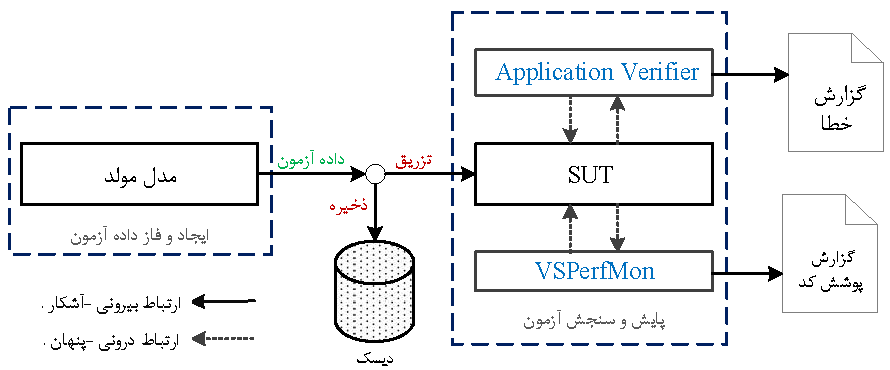
\includegraphics[width=\textwidth, clip=true,  trim= 0 0 0 0]{chapter4/ch4_iust_deep_fuzzer_crop.pdf}
	\caption[معماری فازر قالب فایل پیشنهادی و ارتباط بین مؤلفه‌های مختلف آن]
	{
		معماری فازر قالب فایل پیشنهادی. فازر به‌صورت کاملاً پیمانه‌ای پیاده‌سازی شده است. پیکان‌ها ارتباطات بین مؤلفه‌ها را نشان می‌دهند. ارتباط بیرونی، سازوکار ارتباطی است که توسط ما پیاده‌سازی شده یا قابل تغییر است و ارتباط درونی سازو‌کار ارتباطی است که توسط پیمانه‌های شخص ثالث استفاده می‌شود. 
	}
	\label{ch4_iust_deep_fuzzer_crop.pdf}
	%\ref{ch4_iust_deep_fuzzer_crop.pdf}
\end{figure}




\section{خلاصه}
مدل‌های زبانی عصبی در سطح کاراکتر قابلیت یادگیری یک توزیع آماری روی یک توالی از کاراکترها را دارند. در این فصل ما ساختار یک فایل را به صورت یک توالی از کاراکترها (بایت‌ها) مدل کرده و با ارائه چندین مدل زبانی عصبی و چندین راهبرد تولید داده‌های جدید از این مدل‌ها، یک روش تولید خودکار داده آزمون ارائه دادیم که قابل استفاده در فازرهای قالب فایل مختلف است. ما همچنین دو الگوریتم با عنوان‌های فاز داده عصبی و فاز فراداده عصبی ارائه کردیم. هر کدام از این الگوریتم‌ها بدشکل‌سازی داده آزمون ورودی را با هدف خاصی انجام می‌دهند: اولی با هدف جابه‌جایی داده‌های یک فایل به منظور ایجاد خطا در هنگام پرداخت آنها و دومی با هدف جابه‌جایی فراداده‌های یک فایل برای اینجا خطا در تجزیه‌گر اولیه ساختار فایل تحت فاز. 

در بخش پایانی فصل نیز یک فازر قالب فایل را طراحی و پیاده‌سازی کردیم که از آن می‌توان برای آزمون فازی برنامه‌هایی با ورودی فایل استفاده کرد. خروجی این فازر علاوه بر گزارش خطاهای یافت شده حین فرایند آزمون، گزارش میزان پوشش کد و ذخیره کلیه داده‌های آزمون تولید شده نیز است. معماری فازر پیشنهادی کاملاً پیمانه‌ای بوده و با تعویض پیمانه‌ پایش، امکان استفاده از آن در سیستم‌های عاملی به‌جز ویندوز فراهم می‌شود. فازر معرفی شده یک فازر جعبه خاکستری و مجهز به یک روش تولید داده آزمون ترکیبی است. در فصل \ref{ch:5}، به ارزیابی روش پیشنهادی و بررسی یافته‌های حاصل از آن می‌پردازیم.






